\documentclass[12pt,a4paper, twocolumn]{article}
\usepackage[utf8]{inputenc}
\usepackage{amsmath}
\usepackage{amsfonts}
\usepackage{amssymb}
\usepackage{graphicx}
\usepackage{xcolor}
\usepackage{pgf}
\usepackage{tikz}
\usetikzlibrary{arrows,automata}
\usetikzlibrary{calc}
\usetikzlibrary{positioning}
\usepackage{titlesec}
\usepackage[left=2cm,right=2cm,top=2cm,bottom=2cm]{geometry}
\author{Wael Ali}
\date{}
\title{Abstraction of Graph Theory}
\begin{document}
\newcommand{\hsplit}{\rule{\linewidth}{1pt}\\}

\maketitle
\section*{Section (2)}
\begin{itemize}
\item A \underline{\textbf{simple graph}} $G$ consists of a non-empty finite set $V(G)$ of elements called vertices
(or nodes), and a finite set $E(G)$ of distinct unordered pairs of distinct elements of $V(G)$ called edges.
\item A \underline{\textbf{graph}} $G$ consists of a non-empty finite set $V(G)$ of elements called vertices, and a finite family $E(G)$ of unordered pairs of (not necessarily distinct) elements of $V(G)$ called edges.
\item Two graphs $G1$ and $G2$ are \underline{\textbf{isomorphic}} if there is a one-one correspondence between the vertices of $G_x$ and those of $G2$ such that the number of edges joining any two vertices of $G_x$ is equal to the number of edges joining the corresponding vertices of $G2$ .
	\begin{figure}[h!]
	\centering
	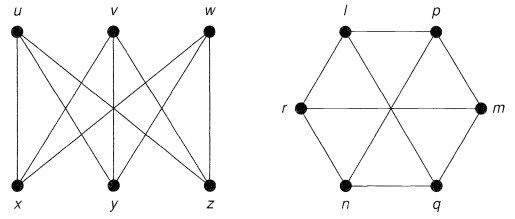
\includegraphics[scale=0.4]{figures/isomorphism1.png}
	\caption{Two simple graphs that are isomorphic to each other}
	\end{figure}
\item A graph is \underline{\textbf{connected}} if it cannot be expressed as the union of two graphs, and \underline{\textbf{disconnected}}.
	\begin{figure}[h!]
	\centering
	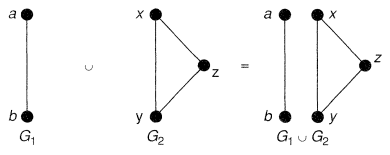
\includegraphics[scale=0.5]{figures/graphUion.png}
	\caption{Each of $G_1$ and $G_2$ is a component of $G_1 \cup G_2$}
	\end{figure}
\item Two vertices $v$ and $w$ of a graph $G$ are \underline{\textbf{adjacent}} if there is an edge $vw$ joining them, and the vertices $v$ and $w$ are then \underline{\textbf{incident}} with such an edge. Similarly, two distinct edges e and/are adjacent if they have a vertex in common.
\item The \underline{\textbf{degree}} of a vertex $v$ of $G$ is the number of edges incident with $v$, and is written $deg(v)$. \emph{Loop}-edge increase node-degree by 2. vertex of degree 0 is an \underline{\textbf{isolated vertex}} and a vertex of degree 1 is an \underline{\textbf{end-vertex}}.
\item \textbf{\underline{Handshaking lemma}}; in any graph the sum of all the vertex-degrees is an even number - in
fact, twice the number of edges, since each edge contributes exactly 2 to the sum.
\item A \textbf{\underline{subgraph}} of a graph $G$ is a graph, each of whose vertices belongs to $V(G)$ and each
of whose edges belongs to $E(G)$.
\item \underline{\textbf{Matrix representation}} one way to represent graph is by its \textbf{adjacency matrix} $A$, and its \textbf{incidence matrix} $M$ as follows;
	\begin{figure}[h!]
	\centering
	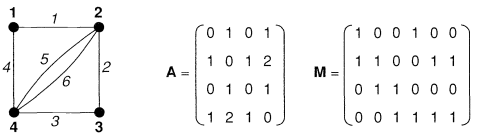
\includegraphics[scale=0.55]{figures/matrixRepresentation.png}
	\end{figure}
\end{itemize}
\newpage
\section*{Exercise 2}
\begin{itemize}
	\item[2a] {\color{blue} Write down the vertex-set and edge-set of each graph in Fig 2.5}
	\begin{figure}[h!]
	\centering
	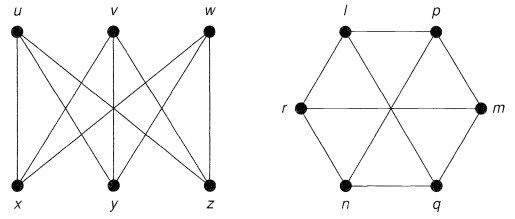
\includegraphics[scale=0.5]{figures/isomorphism1.png}
	\end{figure}
	\hsplit
	
	The first graph $G_1$ is $(V(G_1), E(G_1))$
	\begin{eqnarray*}
	V(G_1) & = & \{ x, y, z, u, v, w\}\\
	E(G_1) & = &	 \{ \{x, u\}, \{x, v\}, \{x, w\}, \\
				  & &    \{y, u\}, \{y, v\}, \{y, w\}, \\ 
				  & &    \{z, u\}, \{z, v\}, \{z, w\} \}
	\end{eqnarray*}
	The second graph $G_2$ is $(V(G_2), E(G_2))$
	\begin{eqnarray*}
	V(G_2) & = & \{ n, m, q, r, l, p\}\\
	E(G_2) & = &	 \{ \{n, r\}, \{n, p\}, \{n, q\}, \\
				  & &    \{m, r\}, \{m, p\}, \{m, q\}, \\ 
				  & &    \{l, r\}, \{l, p\}, \{l, q\} \}
	\end{eqnarray*}
	
	\item[2b] {\color{blue} Draw; \begin{itemize}
			\item[(i)] a simple graph.
			\item[(ii)] a non-simple graph with no loops.
			\item[(iii)] a non-simple graph with no multiple edges, each having 5 vertices each having 5 vertices and 8 edges.
		\end{itemize}}
		\hsplit
		\begin{itemize}
			\item[]
			\begin{figure}[h!]
			\centering 				
			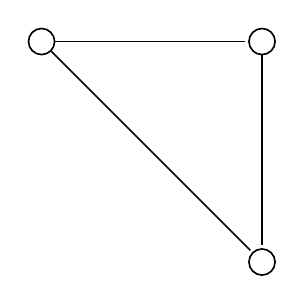
\begin{tikzpicture}[-,>=stealth',shorten >=1pt,auto,node distance=2.8cm,
                    semithick]
 				 \tikzstyle{every state}=[fill=white, draw=black, text=black,  minimum size=0.1pt]
 					 \node[state] (A)                    {};
  					 \node[state]         (B) [right of=A] {};
  					 \node[state]         (C) [below of=B] {};
 					 \path (A) edge (B)
 					 		 	(B) edge (C)
 					 			(A) edge (C);
				\end{tikzpicture}
				\caption{ (i) a simple graph}
			\end{figure}
		\item[]
			\begin{figure}[h!]
			\centering 				
			\			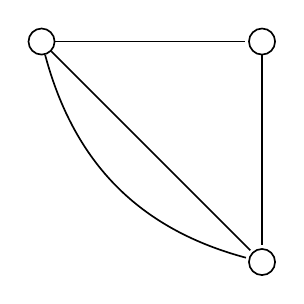
\begin{tikzpicture}[-,>=stealth',shorten >=1pt,auto,node distance=2.8cm,
                    semithick]
 				 \tikzstyle{every state}=[fill=white, draw=black, text=black,  minimum size=0.1pt]
 					 \node[state] (A)                    {};
  					 \node[state]         (B) [right of=A] {};
  					 \node[state]         (C) [below of=B] {};
 					 \path (A) edge (B)
 					 		 	(B) edge (C)
 					 			(A) edge (C)
 					 			(A) edge [bend right] (C);
				\end{tikzpicture}
				\caption{(ii) a non-simple graph with no loops}
			\end{figure}
		\item[]
			\begin{figure}[h!]
			\centering 				
			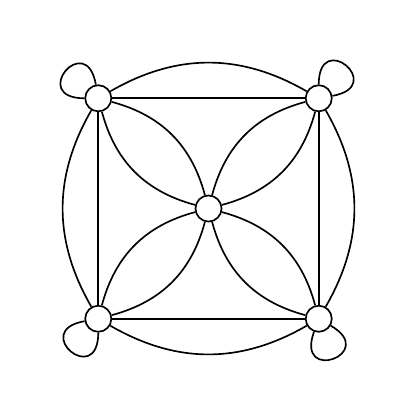
\begin{tikzpicture}[-,auto,node distance=2.8cm,semithick]
 				 \tikzstyle{every state}=[fill=white, draw=black, text=black,  minimum size=0.1pt]
 					 \node[state] (A)                    {};
  					 \node[state]         (B) [right of=A] {};
  					 \node[state]         (C) [below of=B] {};
  					 \node[state]         (D) [below of=A] {};
  					 \node[state]         (E) at ($(D)!0.5!(B)$) {};
 					 \path
 					 			(A) edge (B)
 					 			(A) edge [bend left] (B)
 					 		 	(B) edge (C)
 					 		 	(B) edge [bend left] (C)
 					 			(C) edge (D)
 					 			(C) edge [bend left] (D)
 					 			(A) edge (D)
 					 			(A) edge [bend right] (D)
 					 			(A) edge [bend right] (E)
 					 			(A) edge [bend left] (E)
								(B) edge [bend right] (E)
 					 			(B) edge [bend left] (E)
 					 			(C) edge [bend right] (E)
 					 			(C) edge [bend left] (E)
 					 			(D) edge [bend right] (E)
 					 			(D) edge [bend left] (E);
					%\draw[semithick,-] (A) to [out=10, in=90,loop] (A);
					\draw[semithick,-] (A) to [out=100, in=180,loop] (A); 	
					\draw[semithick,-] (B) to [out=10, in=90,loop] (B);
					%\draw[semithick,-] (B) to [out=100, in=180,loop] (B); 	
					\draw[semithick,-] (C) to [out=-110, in=-30, loop] (C); 	
					\draw[semithick,-] (D) to [out=-170, in=-90, loop] (D); 					 			 					 			
				\end{tikzpicture}
				\caption{(iii) a 5-vertices and 8-degress each}
			\end{figure}			
		\end{itemize}
	\item[2c] {\color{blue} Draw;
		\begin{itemize}
			\item[(i)] Draw a graph on six vertices whose degrees are 5,5,5,5,3,3; does there exist  a simple graph with these degrees?
			\item[(ii)] How does the answer to part (i) changed if the degrees are 5, 5, 4, 3, 3,2?
		\end{itemize}}
		\hsplit
					\begin{figure}[h!]
			\centering 				
			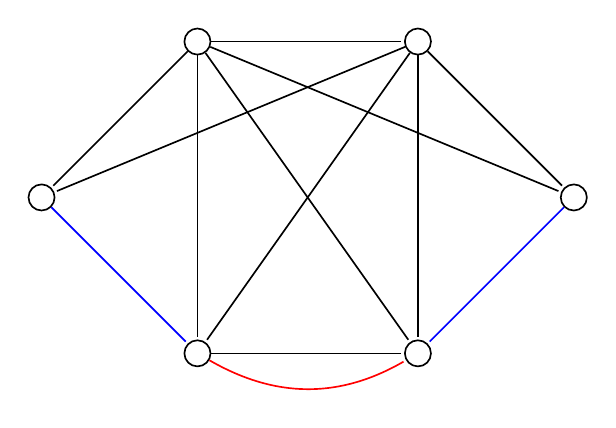
\begin{tikzpicture}[-,>=stealth',shorten >=1pt,auto,node distance=2.8cm, semithick]
 				 \tikzstyle{every state}=[fill=white, draw=black, text=black,  minimum size=0.1pt]
 					 \node[state] 			(A)                    {};
  					 \node[state]         (B) [right of=A] {};
  					 \node[state]         (C) [below left of=A] {};
  					 \node[state] 		  (D) [below right of=B] {};
  					 \node[state]		  (E) [below right of=C] {};
  					 \node[state]		  (F) [below left of=D] {};
  					
 					  \path
 					  			(A) edge (B)
 					 			(A) edge (C)
 					 			(A) edge (D)
 					 			(A) edge (E)
								(A) edge (F) 					 			
 					 			(B) edge (C)
 					 			(B) edge (D)
 					 			(B) edge (E)
 					 			(B) edge (F)
 					 			(E) edge (F)
								(E) edge [bend right, color=red] (F) 					 			
 					 			(C) edge [color=blue] (E)
 					 			(D) edge [color=blue] (F);
				\end{tikzpicture}
				\caption{(i) a non-simple graph with with 6-vertices with degrees [5,5,5,5,3,3]}
			\end{figure}\\
			There isn't a simple graph with last mentioned degrees for a 6-vertices graph. But it we just remove the red-arc and one of the blue-arcs, we then get a simple graph as shown in the next figure. 
			\begin{figure}[h!]
			\centering 				
			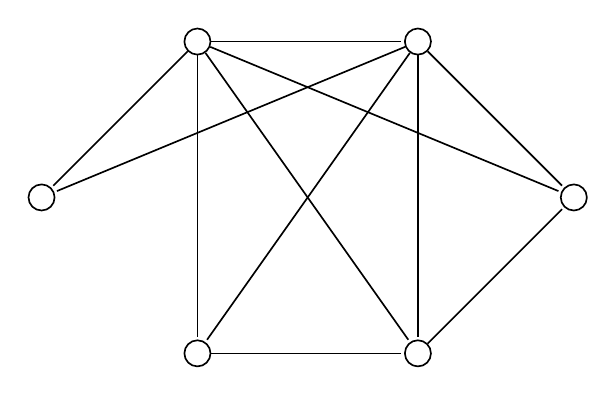
\begin{tikzpicture}[-,>=stealth',shorten >=1pt,auto,node distance=2.8cm, semithick]
 				 \tikzstyle{every state}=[fill=white, draw=black, text=black,  minimum size=0.1pt]
 					 \node[state] 			(A)                    {};
  					 \node[state]         (B) [right of=A] {};
  					 \node[state]         (C) [below left of=A] {};
  					 \node[state] 		  (D) [below right of=B] {};
  					 \node[state]		  (E) [below right of=C] {};
  					 \node[state]		  (F) [below left of=D] {};
  					
 					  \path
 					  			(A) edge (B)
 					 			(A) edge (C)
 					 			(A) edge (D)
 					 			(A) edge (E)
								(A) edge (F) 					 			
 					 			(B) edge (C)
 					 			(B) edge (D)
 					 			(B) edge (E)
 					 			(B) edge (F)
 					 			(E) edge (F)
 					 			(F) edge (D);
				\end{tikzpicture}
				\caption{(i) a simple graph with with 6-vertices with degrees [5,5,4,3,3,2]}
			\end{figure}\\
\item[(2d)] {\color{blue} Verify that handshaking lemma is hold for figure 2.1}
\hsplit
\begin{figure}[h!]
\centering
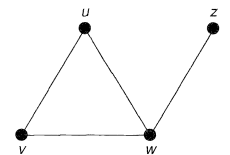
\includegraphics[scale=0.5]{figures/2_d.png}
\end{figure}
As we can see in the last figure, the sum of all vertex-degrees is $2+2+3+1=8$ which is an even number.
\item[(2f)] {\color{blue} \begin{itemize}
	\item[(i)] By suitably lettering the vertices, show that the two graphs in Fig. 2.20 are isomorphic.
	\item[(ii)] Explain why two graphs in Fig. 2.21 are not isomorphic.
\end{itemize}  }
\hsplit
(i) As shown in the following figure \ref{isomorphic} the two graphs are labeled with the same letters in a way to emphasize that they are both isomorphic to each other.
\begin{figure}[h!]
			\centering 				
			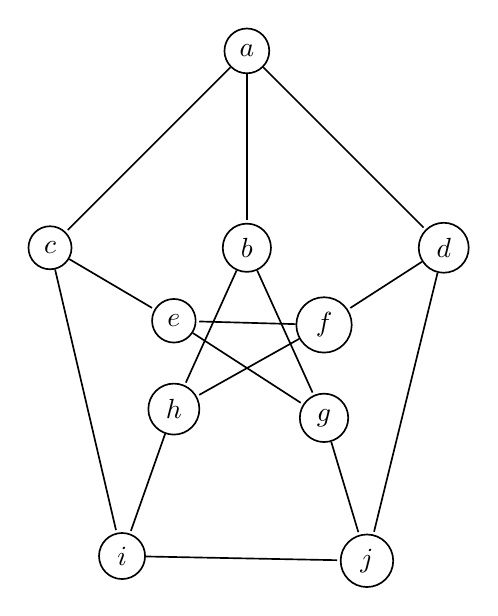
\begin{tikzpicture}[-,>=stealth',shorten >=1pt,auto,node distance=2.5cm, semithick]
 				 \tikzstyle{every state}=[fill=white, draw=black, text=black,  minimum size=0.1pt]
 					 \node[state] 			(A)                    		{$a$};
  					 \node[state]         (B) [below of=A] {$b$};
  					 \node[state]         (C) [left of=B] 		{$c$};
  					 \node[state]         (D) [right of=B] 	{$d$};
					\node[state]		  (E) [below left=0.5cm and 0.5cm of B] {$e$};
					\node[state]		  (F) [below right=0.5cm and 0.5cm of B] {$f$};
					\node[state]		  (G) [below=0.5cm and 0cm of F] {$g$}; 					 
  					 \node[state]		  (H) [below= 0.5cm and 0.5cm of E] {$h$};
  					 \node[state]		  (I)  [below right=3.5cm and 0.5cm of C] {$i$};
  					 \node[state]		  (J)  [below left=3.5cm and 0.5cm of D] {$j$};
 					  \path
 					  			(A) edge (B)
 					 			(A) edge (C)
 					 			(A) edge (D)
 					 			(B) edge (H)
 					 			(B) edge (G)
 					 			(D) edge (F)
 					 			(F) edge (H)
 					 			(C) edge (E)
 					 			(E) edge (G)
 					 			(C) edge (I)
 					 			(H) edge (I)
 					 			(D) edge (J)
 					 			(G) edge (J)
 					 			(F) edge (E)
 					 			(I) edge (J);
				\end{tikzpicture}
			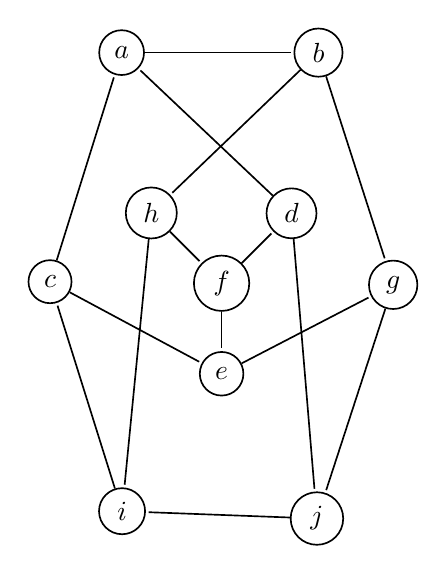
\begin{tikzpicture}[-,>=stealth',shorten >=1pt,auto,node distance=2.5cm, semithick]
 				 \tikzstyle{every state}=[fill=white, draw=black, text=black,  minimum size=0.1pt]
 					 \node[state] 			(A)                    		{$a$};
  					 \node[state]         (B) [right of=A] {$b$};
  					 \node[state]         (C) [below left=2.5cm and 0.5cm of A] 		{$c$};
  					 \node[state]         (D) [below right=2.5cm and 0.5cm of B] 	{$g$};
					\node[state]		  (F) at ($(C)!0.5!(D)$) {$f$};
					\node[state]		  (E) [above left=0.4cm and 0.4cm of F] {$h$};
					\node[state]		  (G) [above right=0.4cm and 0.4cm of F] {$d$};															
					\node[state]		  (H) [below=0.5cm and 0cm of F] {$e$}; 					 
  					 \node[state]		  (I)  [below right=2.5cm and 0.5cm of C] {$i$};
  					 \node[state]		  (J)  [below left=2.5cm and 0.5cm of D] {$j$};
 					  \path
 					  (A) edge (B)
 					  (B) edge (D)
 					  (D) edge (J)
 					  (J) edge (I)
 					  (I) edge (C)
 					  (C) edge (A)
 					  (C) edge (H)
 					  (H) edge (D)
 					  (B) edge (E)
 					  (E) edge (F)
 					  (F) edge (H)
 					  (F) edge (G)
 					  (G) edge (A)
 					  (G) edge (J)
 					  (E) edge (I);
				\end{tikzpicture}
				\caption{(i) }
				\label{isomorphic}
			\end{figure}\\
(ii) As shown in the following figure \ref{notisomorphic}, we cannot find the red part of the first graph as a subset in the second graph.
\begin{figure}[h!]
\centering
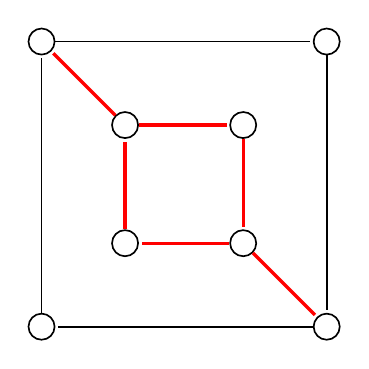
\begin{tikzpicture}[-,>=stealth',shorten >=1pt,auto,node distance=1.5cm, semithick]
 				 \tikzstyle{every state}=[fill=white, draw=black, text=black,  minimum size=0.1pt]
 					 \node[state] 			(A)                    		{};
 					 \node[state] 			(B) [right of=A]                   		{};
 					 \node[state] 			(C) [below of=B]                   		{};
 					 \node[state] 			(D) [below of=A]                  		{};
 					 \node[state]          (E) [above left of=A] {};
 					 \node[state]          (F) [above right of=B] {};
 					 \node[state]          (G) [below right of=C] {};
 					 \node[state]          (H) [below left of=D] {};
				\path
				(A) edge [color=red, very thick] (B)
				(B) edge [color=red, very thick] (C)
				(C) edge [color=red, very thick] (D)
				(D) edge [color=red, very thick] (A)
				(E) edge (F)
				(F) edge (G)
				(G) edge (H)
				(H) edge (E)
				(A) edge [color=red, very thick] (E)
				(C) edge [color=red, very thick] (G);
\end{tikzpicture}
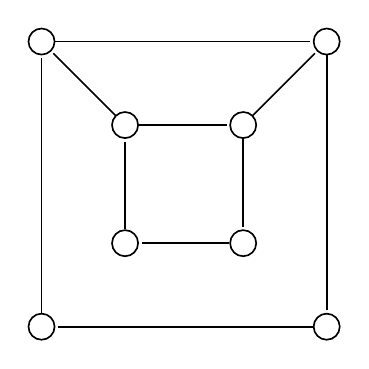
\begin{tikzpicture}[-,>=stealth',shorten >=1pt,auto,node distance=1.5cm, semithick]
 				 \tikzstyle{every state}=[fill=white, draw=black, text=black,  minimum size=0.1pt]
 					 \node[state] 			(A)                    		{};
 					 \node[state] 			(B) [right of=A]                   		{};
 					 \node[state] 			(C) [below of=B]                   		{};
 					 \node[state] 			(D) [below of=A]                  		{};
 					 \node[state]          (E) [above left of=A] {};
 					 \node[state]          (F) [above right of=B] {};
 					 \node[state]          (G) [below right of=C] {};
 					 \node[state]          (H) [below left of=D] {};
				\path
				(A) edge (B)
				(B) edge (C)
				(C) edge (D)
				(D) edge (A)
				(E) edge (F)
				(F) edge (G)
				(G) edge (H)
				(H) edge (E)
				(A) edge (E)
				(B) edge (F);
\end{tikzpicture}
\caption{(ii) not isomorphic graphs}
\label{notisomorphic}
\end{figure}
\end{itemize}
\clearpage 

\section*{Section (3)}
\begin{itemize}
	\item \underline{\textbf{Null graphs}}, a graph whose edge-set is empty. \underline{\textbf{Complete graph}}, a simple graph in which each pair of distinct vertices are adjacent, in this case $k$-vertex must has $n(n-1)/2$ degree as $n$ the total number of vertices.
	\item \underline{\textbf{Regular graph}}, a graph in which each vertex has the same degree. \textbf{Platonic graphs}, formed from the vertices and edges of the five regular (Platonic) solids - the tetrahedron, octahedron, cube.
	\item \textbf{\underline{Bipartite graph}}, If the vertex set of a graph G can be split into two disjoint sets A and B so that each edge of G joins a vertex of A and a vertex of B.  A \textbf{complete bipartite graph} is a bipartite graph in which each vertex in A is joined to each vertex in B by just one edge.
	\item \underline{\textbf{Cubes}}, the $k$-cube $Q_k$ is the graph whose vertices correspond to the sequences ($a_1, a_2, \cdots, a_k$ ), where each $a_i = 0 $ or $1$, and whose edges join those sequences that differ in just one place. You should check that $Q_k$ has $2^{k}$ vertices and $k 2^{k-1}$ edges, and is regular of degree $k$.\\
	\begin{figure}[h!]
	\centering
	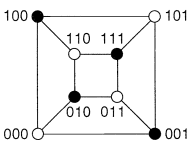
\includegraphics[scale=0.7]{figures/cube1.png}
	\end{figure}
	\item \textbf{\underline{Complement of a simple graph}}, if $G$ is a simple graph with vertex set $V(G)$, its complement $\overline{G}$ is the simple graph with vertex set $V(G)$ in which two vertices are adjacent if and only if they are not adjacent in $G$.
\end{itemize}

\section*{Exercise 3}
\begin{itemize}
	\item[(3a)] {\color{blue} Draw the following graphs:
	\begin{itemize}
		\item[(i)] the null graph $N_5$.
		\item[(ii)] the complete graph $K_6$.
		\item[(iii)] the complete bipartite graph $K_{2,4}$.
		\item[(iv)] the union of $K_{1,3}$ and $W_4$.
		\item[(v)] the complement of the cycle graph $C_4$.
\end{itemize}		
	} 
	\hsplit
		\begin{figure}[h!]
	\centering
	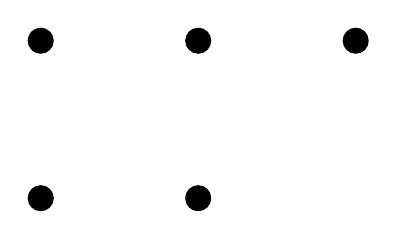
\begin{tikzpicture}[-,auto,node distance=2cm, semithick]
 				 \tikzstyle{every state}=[fill=black, draw=none,  minimum size=0.1pt]
			\node[state]  (1) {};
			\node[state]  (2) [right of=1]{};
			\node[state]  (3) [right of=2]{};		
		 	\node[state]  (4) [below of=1]{};
		 	\node[state]  (5) [below of=2]{};
 	\end{tikzpicture}
 	\caption{(i) Null graph $N_5$}
	\end{figure}
	\begin{figure}[h!]
	\centering
	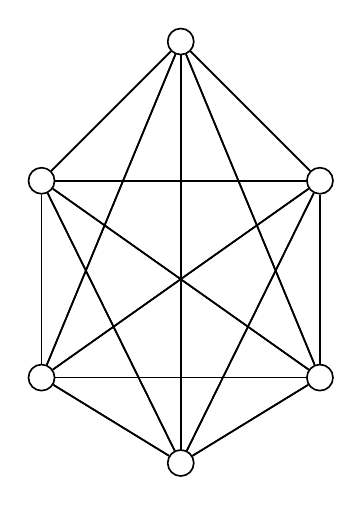
\begin{tikzpicture}[-,auto,node distance=2.5cm, semithick]
 				 \tikzstyle{every state}=[fill=white, draw=black, text=black,  minimum size=0.1pt]
			\node[state]  (1) {};
			\node[state]  (2) [below right of=1]{};
			\node[state]  (3) [below left of=1]{};		
		 	\node[state]  (4) [below of=2]{};
		 	\node[state]  (5) [below of=3]{};
		 	\node[state]  (6) [below=5cm and 0cm of 1]{};
		
		 		\foreach \i in {1,...,6}{
		 		 \foreach \j in {1,...,6}{
		 			\draw  (\i) -- (\j);
		 			}
		 			}
 	\end{tikzpicture}
 	\caption{(ii) Complete graph $K_6$}
	\end{figure}
		\begin{figure}[h!]
	\centering
	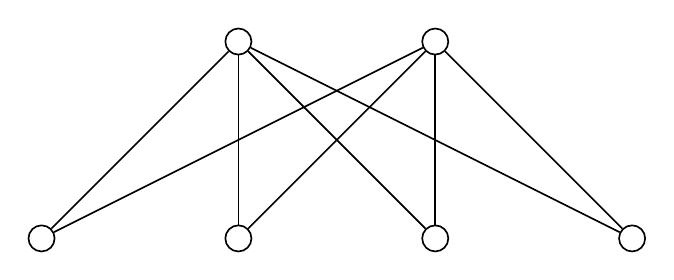
\begin{tikzpicture}[-,auto,node distance=2.5cm, semithick]
 				 \tikzstyle{every state}=[fill=white, draw=black, text=black,  minimum size=0.1pt]
			\node[state]  (A) {};
			\node[state]  (B) [right of=A]{};
			\node[state]  (2) [below of=A]{};
			\node[state]  (1) [left of=2]{};		
		 	\node[state]  (3) [below of=B]{};
		 	\node[state]  (4) [right of=3]{};
		
		 		\foreach \i in {A,...,B}{
		 		 \foreach \j in {1,...,4}{
		 			\draw  (\i) -- (\j);
		 			}
		 			}
 	\end{tikzpicture}
 	\caption{(iii) Complete bipartite graph $K_{2,4}$}
	\end{figure}
		\begin{figure}[h!]
	\centering
	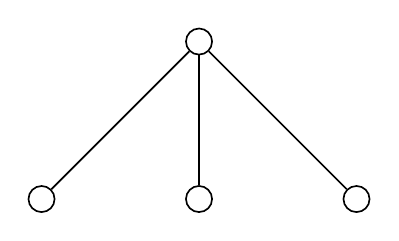
\begin{tikzpicture}[scale=0.8,-,auto,node distance=2cm, semithick]
 				 \tikzstyle{every state}=[fill=white, draw=black, text=black,  minimum size=0.1pt]
			\node[state]  (A) {};
			\node[state]  (2) [below of=A]{};
			\node[state]  (1) [left of=2]{};		
		 	\node[state]  (3) [right of=2]{};
		
		 		 \foreach \j in {1,...,3}{
		 			\draw  (A) -- (\j);
		 			}
 	\end{tikzpicture}
 	  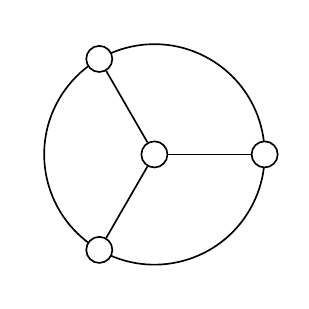
\begin{tikzpicture}[scale=.7, semithick]
 	  \tikzstyle{every state}=[fill=white, draw=black, text=black,  minimum size=0.1pt]
\draw (60:2) arc (60:420:20mm);
    \node[state] (center) at (0,0) {};
\foreach \phi in {1,...,3}{
    \node[state,fill=white] (v_\phi) at (360/3 * \phi:2cm) {};
         \draw (v_\phi) -- (center);
      }
   \end{tikzpicture}
 	\caption{(iv) Union of $K_{1,3}$ and $W_4$}
	\end{figure}
	
	\begin{figure}[h!]
	\centering
	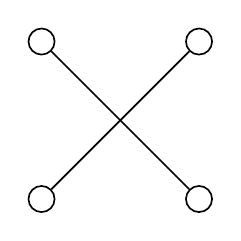
\begin{tikzpicture}[scale=1,-,auto,node distance=2cm, semithick]
 				 \tikzstyle{every state}=[fill=white, draw=black, text=black,  minimum size=0.1pt]
			\node[state]  (A) {};
			\node[state]  (B) [right of=A]{};
			\node[state]  (C) [below of=B]{};		
		 	\node[state]  (D) [below of=A]{};
			\path
				(A) edge (C)
				(B) edge (D);
		\end{tikzpicture}
 	\caption{(iv) Complement of cycle graph $C_4$}
	\end{figure}
	\newpage
\item[(3c)] {\color{blue}Draw the graphs $K_{2,2,2}$, and $K_{3,3,2}$, and write down the number of edges of $K_{3,4,5}$}.
\hsplit
The graphs $K_{2,2,2}$ and $K_{3,3,2}$ are shown in the following figures, respectively.\\
For the graph $K_{3,4,5}$, there is 47 edges. 
\begin{figure}[h!]
\centering
	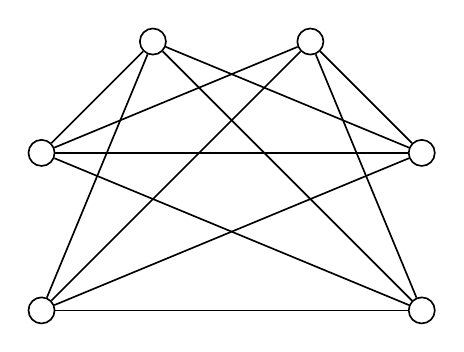
\begin{tikzpicture}[scale=0.6,-,auto,node distance=2cm, semithick]
 				 \tikzstyle{every state}=[fill=white, draw=black, text=black,  minimum size=0.1pt]
			\node[state]  (A) {};
			\node[state]  (B) [right of=A]{};
			\node[state]  (1) [below left of=A]{};		
		 	\node[state]  (2) [below of=1]{};
		 	\node[state] (C) [below  right of=B]{};
		 	\node[state] (D) [below of=C]{};
			
				\foreach \i in {A,...,D}{
		 		 \foreach \j in {1,...,2}{
		 			\draw  (\i) -- (\j);
		 			}
		 			}
		 		\foreach \i in {A,...,B}{
		 		 \foreach \j in {C,...,D}{
		 			\draw  (\i) -- (\j);
		 			}
		 			}
 	\end{tikzpicture}
 	\caption{$K_{2,2,2}$}
\end{figure}
\begin{figure}[h!]
\centering
	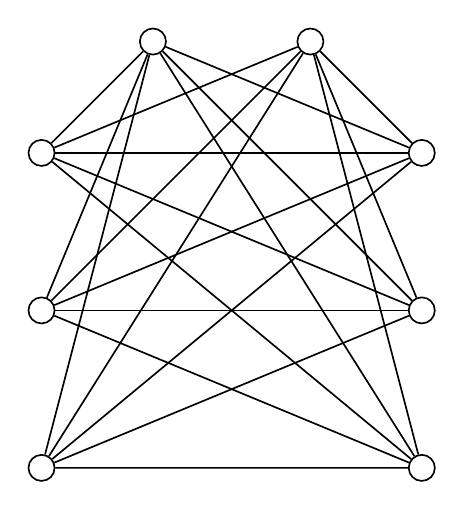
\begin{tikzpicture}[scale=0.6,-,auto,node distance=2cm, semithick]
 				 \tikzstyle{every state}=[fill=white, draw=black, text=black,  minimum size=5pt]
			\node[state]  (A) {};
			\node[state]  (B) [right of=A]{};			
			\node[state]  (1) [below left of=A]{};		
		 	\node[state]  (2) [below of=1]{};
		 	\node[state] (3) [below of=2] {};
		 	\node[state] (C) [below  right of=B]{};
		 	\node[state] (D) [below of=C]{};
		 	\node[state] (E) [below of=D]{};
			
				\foreach \i in {A,...,E}{
		 		 \foreach \j in {1,...,3}{
		 			\draw  (\i) -- (\j);
		 			}
		 			}
		 		\foreach \i in {A,...,B}{
		 		 \foreach \j in {C,...,E}{
		 			\draw  (\i) -- (\j);
		 			}
		 			}
 	\end{tikzpicture}
 	\caption{$K_{3,3,2}$}
\end{figure}
\item[(3g)] {\color{blue} A simple graph that is isomorphic to its complement is self-complementary.
	\begin{itemize}
		\item[(i)] Prove that, if $G$ is self-complementary, then $G$ has $4k$ or $4k+1$ vertices, where $k$ is an integer,
		\item[(ii)] Find all self-complementary graphs with 4 and 5 vertices,
		\item[(iii)] Find a self-complementary graph with 8 vertices.
	\end{itemize}}
	\hsplit
	\begin{itemize}
		\item[(i)] \underline{Proof}\\
			If $G$ is a self-complementary with $n$ vertices, and $$ G \cup \overline{G} =  K_n.$$ But we know that, the total number of edge in the complete graph $K_n$ i.e. $|E(K_n)| $is $n(n-1)/2$, that is, $$|E(G)| =  |E(\overline{G})| = \frac{n(n-1)}{4}.$$ In other words, $n$ or $n-1$ must be divisible by 4, that is, when $n$ is $4k$ or $4k+1$.
			\item[]
			\begin{figure}[h!]
			\centering
				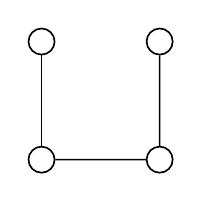
\begin{tikzpicture}[scale=0.4,-,auto,node distance=1.5cm, semithick]
 				 \tikzstyle{every state}=[fill=white, draw=black, text=black,  minimum size=5pt]
						\node[state]  (A) {};
						\node[state] (B) [below of=A]{};
						\node[state] (C) [right of=B]{};
						\node[state] (D) [above of=C]{};
						
						\path
							(A) edge (B)
							(B) edge (C)
							(C) edge (D);
			
 				\end{tikzpicture}
 				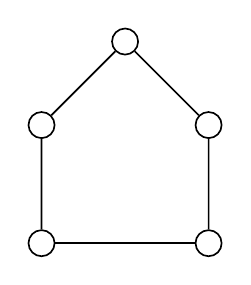
\begin{tikzpicture}[scale=0.4,-,auto,node distance=1.5cm, semithick]
 				 \tikzstyle{every state}=[fill=white, draw=black, text=black,  minimum size=5pt]
						\node[state]  (A) {};
						\node[state] (B) [below left of=A]{};
						\node[state] (C) [below right of=A]{};
						\node[state] (D) [below of=B]{};
						\node[state] (E) [below of=C]{};
						
						\path
							(A) edge (B)
							(A) edge (C)
							(B) edge (D)
							(C) edge (E)
							(D) edge (E);
			
 				\end{tikzpicture}
 				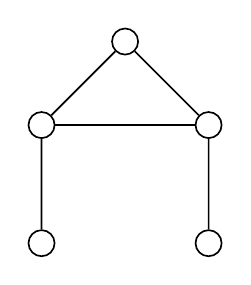
\begin{tikzpicture}[scale=0.4,-,auto,node distance=1.5cm, semithick]
 				 \tikzstyle{every state}=[fill=white, draw=black, text=black,  minimum size=5pt]
						\node[state]  (A) {};
						\node[state] (B) [below left of=A]{};
						\node[state] (C) [below right of=A]{};
						\node[state] (D) [below of=B]{};
						\node[state] (E) [below of=C]{};
						
						\path
							(A) edge (B)
							(A) edge (C)
							(B) edge (D)
							(C) edge (E)
							(B) edge (C);
			
 				\end{tikzpicture}
				\caption{(ii) 4 and 5 vertices self-complementary graphs}
			\end{figure}
			\begin{figure}[h!]
			\centering
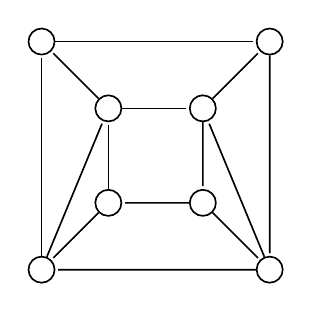
\begin{tikzpicture}[scale=.8,-,>=stealth',shorten >=1pt,auto,node distance=1.2cm, semithick]
 				 \tikzstyle{every state}=[fill=white, draw=black, text=black,  minimum size=0.1pt]
 					 \node[state] 			(A)                    		{};
 					 \node[state] 			(B) [right of=A]                   		{};
 					 \node[state] 			(C) [below of=B]                   		{};
 					 \node[state] 			(D) [below of=A]                  		{};
 					 \node[state]          (E) [above left of=A] {};
 					 \node[state]          (F) [above right of=B] {};
 					 \node[state]          (G) [below right of=C] {};
 					 \node[state]          (H) [below left of=D] {};
				\path
				(A) edge (B)
				(B) edge (C)
				(C) edge (D)
				(D) edge (A)
				(E) edge (F)
				(F) edge (G)
				(G) edge (H)
				(H) edge (E)
				(A) edge (E)
				(B) edge (F)
				(C) edge (G)
				(D) edge (H)
				(G) edge (B)
				(H) edge (A);
\end{tikzpicture}
\caption{(iii) a self-complementary graph with 8 vertices}
			\end{figure}
	\end{itemize}
\end{itemize}

\end{document}

